% IEEE standard conference template; to be used with:
%   spconf.sty  - LaTeX style file, and
%   IEEEbib.bst - IEEE bibliography style file.
% --------------------------------------------------------------------------

\documentclass[letterpaper]{article}


\usepackage{spconf,amsmath,amssymb,graphicx}
\usepackage{ucs}
\usepackage[utf8x]{inputenc}
\usepackage[english]{babel}

% Example definitions.
% --------------------
% nice symbols for real and complex numbers
\newcommand{\R}[0]{\mathbb{R}}
\newcommand{\C}[0]{\mathbb{C}}

% bold paragraph titles
\newcommand{\mypar}[1]{{\bf #1.}}

% monospace text
\makeatletter
\DeclareRobustCommand\ttfamily
        {\not@math@alphabet\ttfamily\mathtt
         \fontfamily\ttdefault\selectfont\hyphenchar\font=-1\relax}
\makeatother
\DeclareTextFontCommand{\mytexttt}{\ttfamily\hyphenchar\font=45\relax}

% Title.
% ------
\title{Escape Analysis for Multi-Threaded Javali}
%
% Single address.
% ---------------
\name{Andrei Pârvu, Sebastian Wicki}
\address{Department of Computer Science\\ ETH Z\"urich\\Z\"urich, Switzerland}

% For example:
% ------------
%\address{School\\
%    Department\\
%    Address}
%
% Two addresses (uncomment and modify for two-address case).
% ----------------------------------------------------------
% \twoauthors
 % {A. Andri Parvu, B. Sebastian Wicki}
  %    {ETH Zurich\\
  %    Department of Computer Science}
 % {C. Author-three, D. Author-four\sthanks{The fourth author performed the work
  %    while at ...}}
  %    {School C-D\\
  %    Department C-D\\
  %    Address C-D}


\begin{document}
%\ninept
%
\maketitle
%

\begin{abstract}
Describe in concise words what you do, why you do it (not necessarily
in this order), and the main result.  The abstract has to be
self-contained and readable for a person in the general area. You
should write the abstract last.
\end{abstract}

\section{Introduction}\label{sec:intro}

The basis of this project is an extended version of Javali with support for
basic multi-threading, similar to Java's built-in \texttt{Thread} class. 
Additionally, we also added support for synchronization though locks. Having
those additional language features also give more margin for potential
optimizations, which we will discuss in the following paragraphs.

\mypar{Motivation} 

Escape analysis can determine if an object reference escapes a certain dynamic
scope, for example the scope of a thread or the scope of a stack frame. This
information can be useful for a class of optimizations. In this project, we
explored two optimizations: Stack allocation of objects and synchronization
elision. Since Javali does not support modules or other forms of dynamic code
loading, we can perform a whole-program escape analysis, typically yielding more
precision.

In standard Javali, all non-primitive objects are allocated on the heap. The
existing implementation even leaks those objects, as there is currently on
garbage collection. Using escape analysis, the compiler can infer that certain
objects will never outlive the current stack frame, thus those objects could
be allocated on the stack. This has the advantage that the object will be cleaned
up automatically once the function returns. Additionally, allocating data on the
stack is typically faster than calling \texttt{malloc()} for heap allocation.
This is especially true in multi-threaded programs, as the implementation of
\texttt{malloc()} internally needs to synchronize as well, although modern
implementations such as \texttt{TCMalloc} optimize this case heavily. % TODO TCMalloc ref

In this paper we provide an extended escape analysis for stack allocation that
even allows stack allocation for objects that are shared with other threads,
under the condition that the thread does not outlive the current function.
This is often the case in the fork-join programming model, where a function
forks multiple child threads to work on in parallel on some data, and then
waits for them to join.

As a second optimization, we implement synchronization removal on objects that
never escape the current thread, i.e. that are never shared among multiple threads
thus do not to be locked in order to be accessed safely. 

This optimization is useful for classes that are is written to be thread-safe,
i.e. use synchronization to ensure correctness, but are actually never used
in a multi-threaded setting, which leads to unnecessary overhead. Library
classes such as Java's \texttt{Vector} or \texttt{Hashtable} class are examples
of thread-safe library classes that were later replaced with non-synchronized
alternatives (namely \texttt{ArrayList} and \texttt{HashMap}) for better
performance.

\mypar{Related work} Next, you have to give a brief overview of
related work. For a report like this, anywhere between 2 and 8
references. Briefly explain what they do. In the end contrast to what
you do to make now precisely clear what your contribution is.

\section{Background}\label{sec:background}

Give a short, self-contained summary of necessary
background information. For example, assume you present an
implementation of sorting algorithms. You could organize into sorting
definition, algorithms considered, and asymptotic runtime statements. The goal of the
background section is to make the paper self-contained for an audience
as large as possible. As in every section
you start with a very brief overview of the section. Here it could be as follows: In this section 
we formally define the sorting problem we consider and introduce the algorithms we use
including a cost analysis.

\mypar{Sorting}
Precisely define sorting problem you consider.

\mypar{Sorting algorithms}
Explain the algorithm you use including their costs.

As an aside, don't talk about "the complexity of the algorithm.'' It's incorrect,
problems have a complexity, not algorithms.


\section{Your Proposed Method}\label{sec:yourmethod}

Now comes the ``beef'' of the report, where you explain what you
did. Again, organize it in paragraphs with titles. As in every section
you start with a very brief overview of the section.

In this section, structure is very important so one can follow the technical content.

Mention and cite any external resources that you used including libraries or other code.

\section{Experimental Results}\label{sec:exp}


\mypar{Experimental setup} For the experiments we used two different machines. The first one, running
Ubuntu 14.04 with a i5-3317U, 1.70GHz processor and 4Gb RAM.

We tried to analyze three different aspects of our project: firstly, the running time improvement of just allocating
the unescaped objects on the stack. Secondly, we wanted to see the time benefit of working with stack-allocated
objects instead of heap-allocated ones. And thirdly, we tried to observe the how lock-removal affects single-threaded
programs.\\

\mypar{Results}
For the first experiment, we just allocated various objects without using them afterwards, in order to see how the running time differs
for both cases. TODO: run the actual experiment :)\\

In the second experiment, we wrote a basic matrix multiplication program with the intent of observing how execution time changes when using
stack allocation. The results can be seen in Figure~\ref{fig:matrixmul}. It can be observed that the stack allocation improves running
time with almost 20\%, with the obvious draw-back that more stack memory is used.\\

For the third experiment, we implemented a hash map, which simulates string hashing (because Javali doesn't have strings we used ASCII arrays).
The hash map is implemented to be thread-safe, so we ran the experiment with one thread and lock removal. Results can be seen in Figure~
\ref{fig:hash}; with lock removal, running time is approximately 10\% faster than the unanalyzed version.\\

\begin{figure} \center
%  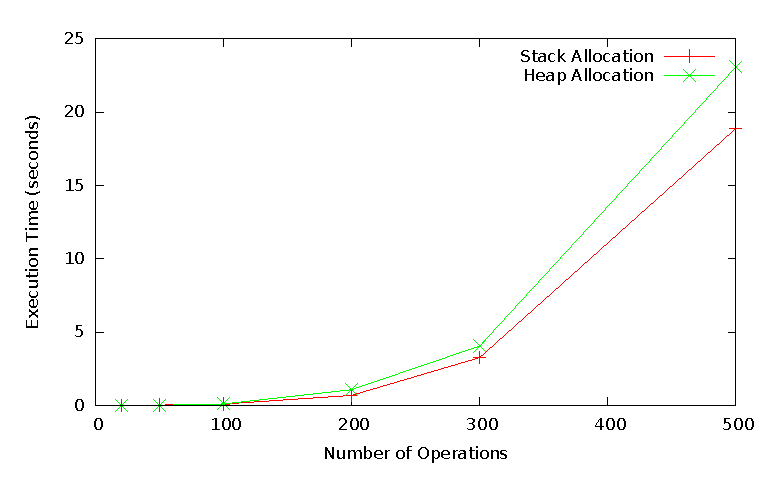
\includegraphics[width=0.8\linewidth]{../Project/results_matrix_mul.eps}
  \caption{Running times matrix multiplication}
  \label{fig:matrixmul}
\end{figure}

\begin{figure} \center
%  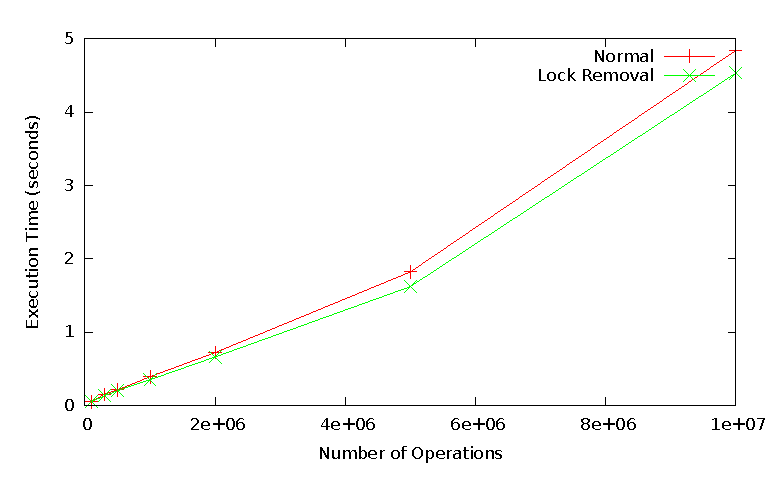
\includegraphics[width=0.8\linewidth]{../Project/results_hash.eps}
  \caption{Running times hash map}
  \label{fig:hash}
\end{figure}

{\bf Comments:}
\begin{itemize}
\item Create very readable, attractive plots (do 1 column, not 2 column plots
for this report) with readable font size. However, the font size should also not be too large; typically it is smaller than the text font size.
An example is in Fig.~\ref{fftperf} (of course you can have a different style).
\item Every plot answers a question. You state this question and extract the
answer from the plot in its discussion.
\item Every plot should be referenced and discussed.
\end{itemize}

\begin{figure}\centering
  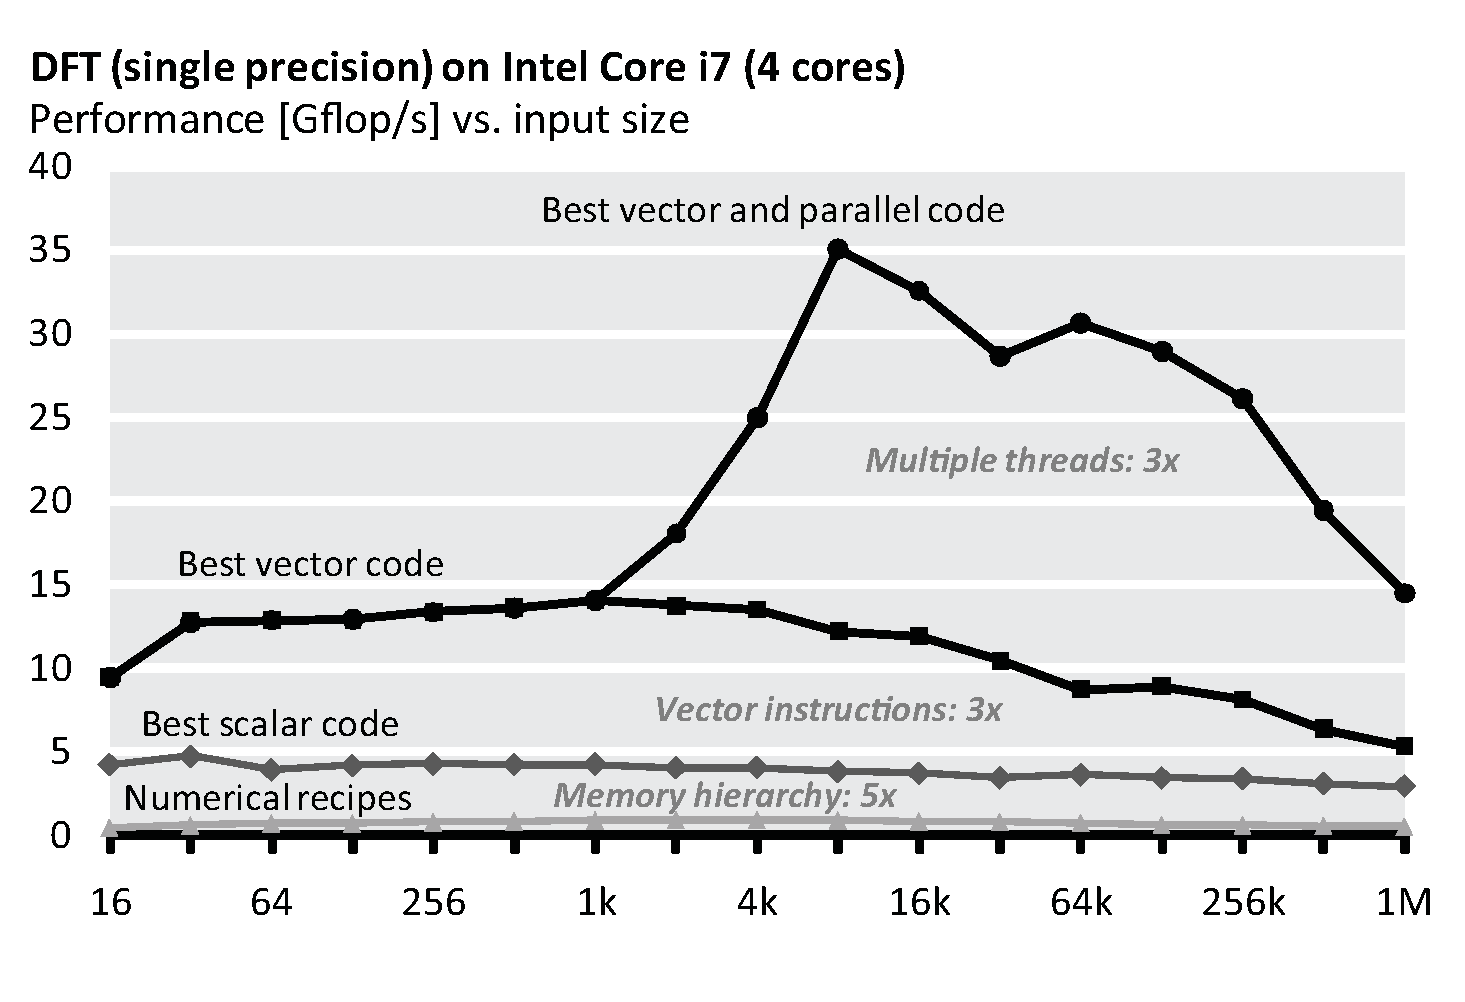
\includegraphics[scale=0.33]{dft-performance.eps}
  \caption{Performance of four single precision implementations of the
  discrete Fourier transform. The operations count is roughly the
  same. The labels in this plot are maybe a little bit too small.\label{fftperf}}
\end{figure}

\section{Conclusions}

Here you need to summarize what you did and why this is
important. {\em Do not take the abstract} and put it in the past
tense. Remember, now the reader has (hopefully) read the report, so it
is a very different situation from the abstract. Try to highlight
important results and say the things you really want to get across
such as high-level statements (e.g., we believe that .... is the right
approach to .... Even though we only considered x, the
.... technique should be applicable ....) You can also formulate next
steps if you want. Be brief. After the conclusions there are only the references.

\section{Further comments}

Here we provide some further tips.

\mypar{Further general guidelines}

\begin{itemize}
\item For short papers, to save space, I use paragraph titles instead of
subsections, as shown in the introduction.

\item It is generally a good idea to break sections into such smaller
units for readability and since it helps you to (visually) structure the story.

\item The above section titles should be adapted to more precisely
reflect what you do.

\item Each section should be started with a very
short summary of what the reader can expect in this section. Nothing
more awkward as when the story starts and one does not know what the
direction is or the goal.

\item Make sure you define every acronym you use, no matter how
convinced you are the reader knows it.

\item Always spell-check before you submit (to us in this case).

\item Be picky. When writing a paper you should always strive for very
high quality. Many people may read it and the quality makes a big difference.
In this class, the quality is part of the grade.

\item Books helping you to write better: \cite{Higham:98} and \cite{Strunk:00}.

\item Conversion to pdf (latex users only): 

dvips -o conference.ps -t letter -Ppdf -G0 conference.dvi

and then

ps2pdf conference.ps
\end{itemize}

\mypar{Graphics} For plots that are not images {\em never} generate the bitmap formats
jpeg, gif, bmp, tif. Use eps, which means encapsulate postscript. It is
scalable since it is a vector graphic description of your graph. E.g.,
from Matlab, you can export to eps.

The format pdf is also fine for plots (you need pdflatex then), but only if the plot was never before in the format 
jpeg, gif, bmp, tif.


% References should be produced using the bibtex program from suitable
% BiBTeX files (here: bibl_conf). The IEEEbib.bst bibliography
% style file from IEEE produces unsorted bibliography list.
% -------------------------------------------------------------------------
\bibliographystyle{IEEEbib}
\bibliography{report}

\end{document}
like
